% !TEX root = ../report.tex
\chapter{Requirements}
\label{ch:requirements}
This chapter discusses the stakeholder of the system. This information helps us to be able to properly write use cases. These will be used to extract the functional requirements. Afterwards, a risk assessment will take place, to ensure that the project is not at great risk.

% Moved to chapter 1
% \section{Vision}

% \begin{figure}[H]
% 	\centering
% 	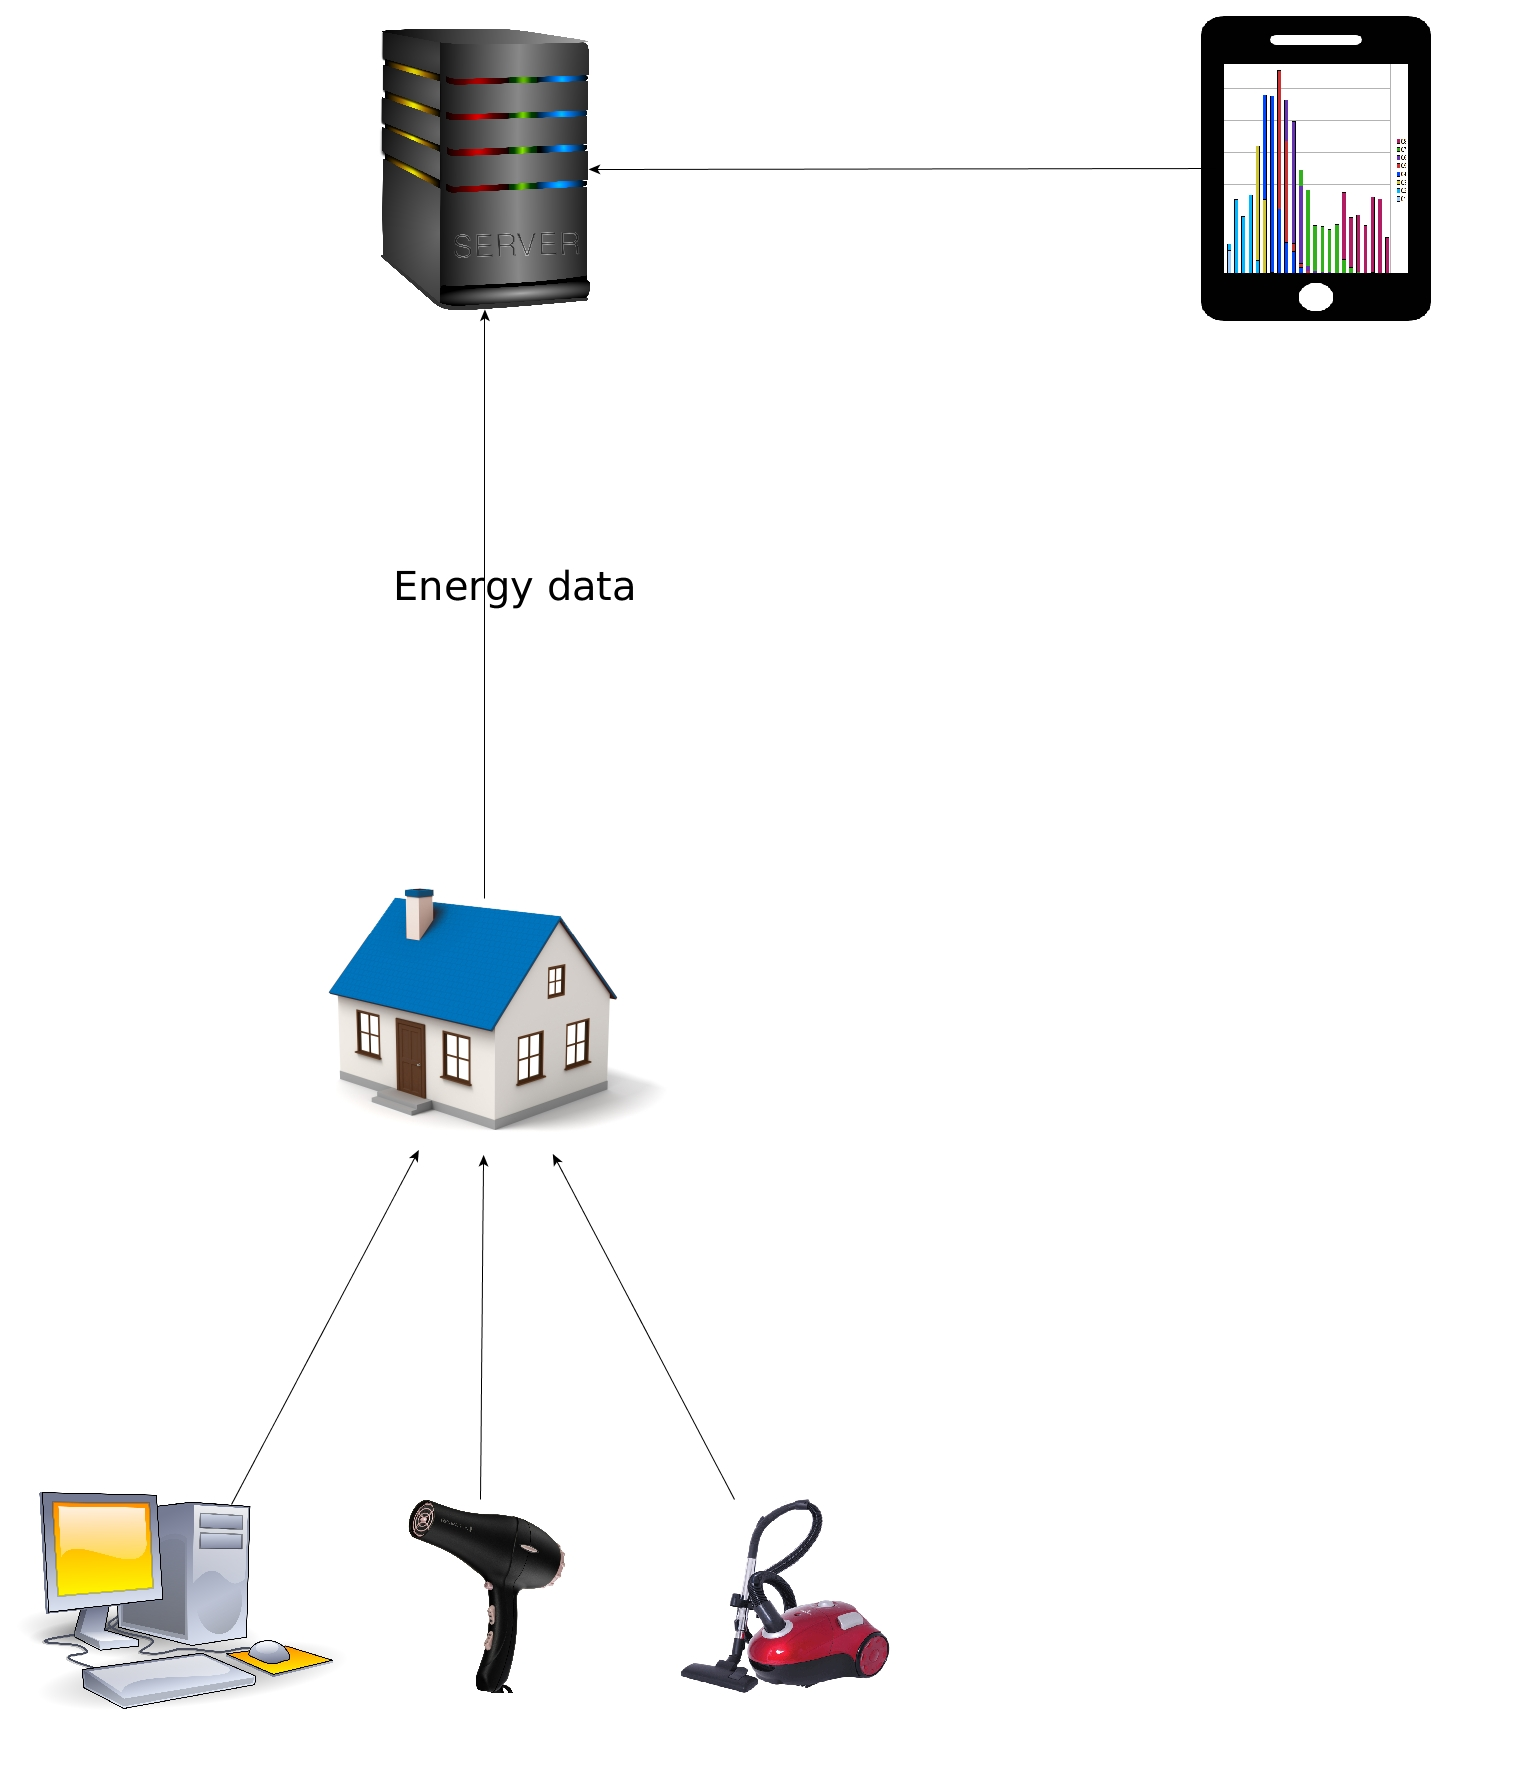
\includegraphics[width=0.7\textwidth]{3-requirements/images/vision.jpg}
% 	\caption{Architectural vision}
% 	\label{fig:vision}
% \end{figure}

%%!TEX root = ../report.tex
\section{Architectural vision}
\label{sec:archvision}


%!TEX root = ../report.tex
\section{Stakeholders and their concerns}

%kind of QA's (accourding to "Software Requirements" 3rd edition, Karll Wiegers and Joy Beatty)
%from page 263:

This section defines all stakeholders of our system and describes the concerns of the stakeholders. A stakeholder is a person, group of persons, or organization that are involved in our system. There are ten stakeholders, ranged from first parties to third parties stakeholders. Several quality standards from the "Software Requirements" book by Microsoft \cite{wiegers2013software} are used. Those quality standards are described in \autoref{table:qa_standard}.

\begin{table}[!htbp] \centering
	\caption{Quality attributes of Software Architecture from "Software Requirements" Book \cite{wiegers2013software}.}
	\label{table:qa_standard}
	\begin{tabular}{L{\tw{0.2}} L{\tw{0.4}}}
		\toprule
		\textbf{Quality Attributes} & \textbf{Brief description}                                                                                        \\ \midrule
		Interoperability            & How easily the system can interconnect and exchange data with other systems or components                         \\
		Reliability                 & How reliable the results of the system are (accuracy). This includes availability, which is the extent to which the system's services are available when and where they are needed \\
		Security                    & How well the system protects against unauthorized access to the application and its data                          \\
		Usability                   & How easy it is for people to learn, remember, and use the system                                                  \\
		Maintainability             & How efficient and effective the system can be maintained/modified by the maintainers \\
		\bottomrule
	\end{tabular}
\end{table}

There are six quality attributes, as can be seen in \autoref{table:qa_standard}, for measuring stakeholders' concern regarding our system.  The stakeholders are listed below and are then explained in more detail below.

\begin{itemize}
%\item Product owner
\item Developers
\item Maintainers
\item Government
\item Home owners
\end{itemize}

\begin{description}

%\item [Product owner] is the owner of the system. This stakeholder funds the project.  This affects the quality attributes usability and availability.

\item [Developers] have to make sure the system provides the functionality that the users expect the system to have. They want the external components (sensors) to work with the system. This means that their main concern is interoperability, because users will want to connect any energy consuming device to this site in order to monitor the consumption.

\item [Maintainers] are mainly concerned that the website is up and running at all times. Meaning their concern is the reliability of the system. Since they are responsible for the maintenance to the system, they also care about its maintainability.

\item [The government] wants to lower the energy consumption of the citizens. It wants to comply with the aims of the EU to reduce the energy consumption by 20\% by 2020. Their main concern is that the end users will be able to use the system, so it will be widely adopted. This means they care about the usability and reliability of the system, because the system is only useful to the government if it is used by allot of people and the statistics of the system are reliable.

\item [Home owners] want to get an insight in their energy usage. They want to know how to effectively reduce their energy consumption. In order to do this, they might want to receive alerts about sudden increases of energy consumption in certain devices. These alerts have to be accurate and reliable. The main concern of the home owners, thus, is the usability of the system.

\end{description}


\autoref{table:stakeholder_concern} illustrates the stakeholder concern matrix. In our approach every stakeholder is equally important. 

\begin{table}[!htbp] \centering
	\caption{Matrix of stakeholders concern.}
	\label{table:stakeholder_concern}
	\begin{tabular}{@{} cl*{8}c @{}}
		&  & \multicolumn{6}{c}{\textbf{Concerns}} \\[2ex]
		& \textbf{Stakeholder} & \rot{Weight} & \rot{Usability} & \rot{Reliability} & \rot{Interoperability} 
		&   \rot{Maintainability} \\
		\cmidrule[1pt]{2-7}		
		 %                	      weight usa  reli  int  r main
		  %& Product owner          & 1 &     &    &     &    & & \\
		  & Developers             & 1 &     &    & 100 &     & & \\
		  %& Sensor suppliers       & 1 &   &  &  &   &    & \\
		  & Maintainers            & 1 &   & 50   &       & 50 &  \\
		  & Government             & 1 & 60  & 40 &        &&  \\
		  & Home owners            & 1 & 70  & 30  &        &&  \\
		\cmidrule{2-7}
		  & Total                  &   & 130 & 120& 100 & 50 &  \\
		\cmidrule{2-7}
	\end{tabular}
\end{table}



% !TEX root = ../report.tex
\section{Key-drivers}
The stakeholder analysis of the previous section leads to the following key drivers:
\begin{itemize}
	\item \req{kd}-- Usability
	\item \req{kd}-- Reliability
	\item \req{kd}-- Interoperability
\end{itemize}


\begin{description}

\item [Usability] has to be the main focus of the system. Users will want to stick to using our system if the usability is better then similar systems of the competitors. Even if competitors have a better availability and or even reliability, there is a good chance that customers will stick to this system if the usability is better. 

\item [Reliability] is very important, because for this kind of system the trust everyone has is crucial. Making the stakeholders trust the system is the most important aspect of this system. If the system at some points does not provide reliable data, without specifically informing about it, then the all the information from the system will be useless.
This not necessarily mean that the system has to be very precise in calculating the statistics. It just has to be very clear about how inaccurate the data is.

\item [Interoperability] is important because in order for the system to be useful to the user, it has to collect and process the energy consumption of devices. All the different homes have different devices who each have a different set of relevant statistics to be calculated.
The sensor data will be monitored with a energy monitoring plug. However, to be able to receive valuable statistics from this data, the system needs to be able to cope with different types of devices.
%
%if the system isn't up at the times when it should, users will lose trust in the system. If a user set an alarm on a device, alarming them if the device exceeds a certain energy consumption, then ideally that alarm has to go any time the device indeed exceeds the given limit of energy consumption.

\end{description}

%!TEX root = ../report.tex

\clearpage
\section{High-level requirements}
The high-level requirements describe the high-level functionality of the system. The high-level requirements are used to derive the functional requirements in section~\ref{sec:functional-requirements}. The high-level requirements are also used to classify the severity of the risks in section~\ref{sec:risk-assesment}. 

This table uses different priorities. First there is the `must' priority, this requirement is an absolute must. The system could not function without the `must' requirement. Besides `must' there is the `should' priority. This priority is highly desirable for the system, but the system could function without this requirement. The last priority is `could', these requirements are nice to have but not really necessary for the core functionality of the system. These different priorities are used through the rest of the document.

\begin{longtable}{L{0.1\textwidth} L{0.12\textwidth} L{0.78\textwidth}}
	\textbf{Nr.} & \textbf{Prio} & \textbf{Description} \\
		
	\hlReqRow{collecting}{Must}{Collecting electricity usage data}
	{ The system must collect electricity usage data, which has to be stored so it can be used to compute statistics and detect changes in energy usage. }
	
	\hlReqRow{analyzing}{Must}{Computing usage statistics}
	{ The system must be capable of computing statistics about the energy usage, like total usage per month, but also periods of peak energy usage. It has to be able to compute such statistics not only per house, but also for individual devices. }
	
	\hlReqRow{analyzing}{Must}{Displaying usage data / statistics}
	{ Data which has been gathered and statistics that have been computed must be displayed to the user in an understandable way. One of the main goals of the system is to make users of the system aware about their energy usage. The data and statistics should be displayed in a way that is intuitive and easy to understand for average consumers. }
	
	\hlReqRow{configuration}{Must}{Configuring the system}
	{ The users of the system must be able to configure the system, i.e. register their house/add new devices/subscribe to alerts etc., using the web interface. This web interface should be user-friendly and intuitive, such that an average consumer is able to use it. }
			    
	\bottomrule

\caption{High Level Requirements}
\label{table:high-level-requirements}	    
\end{longtable}


%!TEX root = ../report.tex
\clearpage
\section{Stories and use-cases}

In this section the architectural significant ue-cae will be presented.

% Installation ?
% Collect and store energy consumption
% The End-Uer wants to display his bill ( to specific ? ) / his energy conumption
% Update ?
% Computation ? by Spark , Map/Reduce , DOES THE SYSTEM COMPUTE THE STATISTICS ONLY WHEN THE USER ASKS FOR PECIFIC STATITICS OR EVERYTIME ?



\textbf{The End user registration} \\
\textit{Number} : UC-1 \\
\textit{Goal} : The user has to register on the website to create his account.
\textit{Primary Actor }:  End-User \\
\textit{Precondition}: The website has the internal process to add an user to the database
\textit{Main Success Scenario }: \\
 1. The user acess the HEMS URL \\
 2. The user click on the " Sign up " Button \\
 3. The website display a regitration form requests the Fullname, Username, email adress and adress of the user.\\
 4. The system checks if the user isn't already in the database. \\
 5. If not the user is added in the database. \\
 6. The user receives a confirmation link on his email adress and clicks on it. \\ % or verification code ?
 7. The user is redirected to the HEMS webite. \\
\textit{Extensions} 1. The user isn't added to the system database. \\
1a. An error message is displayed " The regitration failed, do you want to try again Y/N? ".
1a. If yes Go to step 3.
%2. The user is already in the database.
\textit{Postcondition} : The account is created : the user get acces to his own Home Energy Monitor interface. \\

\textbf{Receive / Collect external energy data} \\% (out of scope ?) \\
\textit{Number}: UC-2 \\
\textit{Goal}: The sytem needs to receive energy data to make the analysis. \\
\textit{Primary Actor} : The system \\
\textit{Precondition}: The energy data is available. \\
\textit{Main Success Scenario}: \\ % what is the process ?
\textit{Extensions} \\
\textit{Post condition}: \\

\textbf{Store energy consumption}\\
\textit{Number} : UC-3 \\
\textit{Goal}: The system needs to store the energy data it just received. \\
\textit{Primary Actor}: System \\
\textit{Precondition} : 1. The system can receive the data. \\
2.The sytem has a database \\
\textit{Main Success Scenario} : 1. The data received is directly stored in the database. \\
\textit{Extensions} : The data isn't stored. % why ? \\
\textit{Post-condition}: The data is in the database.\\

\textbf{Display the next bill}\\
\textit{Number} : UC-4 \\
\textit{Goal}: The End-Uer wants to display the estimation of his next bill \\ 
\textit{Primary Actor}:  End-User \\
\textit{Pre-condition}: The user is registered in the database of the system.\\
\textit{Main Success scenario} : \\
1. The user gets acess to his interface by clicking on "Sign in" Button\\ % sign up ?
2. In the menu he clicks on the "Bill" button.\\
3. In the bill section the user chooses the "Next bill". \\ % the previous ones are alo available
\textit{Extensions} \\
% Authentification failed
\textit{Postcondition} : The bill is displayed.

\textbf{Display analysis, daily/weekly/monthly report}\\ % too generic ?
\textit{Number} : UC-5 \\
\textit{Goal}: The End-Uer wants to display several kind of analysis about hi energy consumption \\ 
\textit{Primary Actor}: End-User \\
\textit{Pre-condition}: The user is registered in the system.
\textit{Main Success scenario} : \\
1. The user gets acess to his interface by clicking on " Sign in " Button \\
2. In the menu he clicks on " Analyis- Chart " \\ 
3. The system computes/make the analysis. \\
\textit{Extensions} : The statistics aren't made. \\
\textit{Postcondition} : Charts with different item are displayed.

\textbf{Update}\\
\textit{Number}: UC-6 \\
\textit{Goal}: The sytem needs to update itself. \\
\textit{Primary Actor} : The system \\
\textit{Precondition}: \\
\textit{Main Success Scenario}: \\
\textit{Extensions} \\
\textit{Post condition}: \\

\textbf{Configuration} \\
\textit{Number}: UC-7\\
\textit{Goal}: The user must be able to configure the sytem with his own characteritics. \\
\textit{Primary Actor} : The user \\
\textit{Precondition}: The user is registered in the database of the system. \\
\textit{Main Success Scenario}: 1. On the dashboard/website the user clicks on the " Settings " button. \\
2. The user gets access to the Settings section with all the possibilities/internal sections for example :frequency of alert, adding new devices etc.\\
\textit{Extensions}:1. The system didn't take into account the information the user just added. \\
1a. An error mesage is displayed " Configuration failed, would you like to try again Y/N ? ". \\
If yes Go to step1. \\
\textit{Post condition}:The system is set with the user's characteritics of his home and preferences. \\

%!TEX root = ../report.tex
\newpage
\section{Functional requirements}
\label{sec:functional-requirements}

% !TEX root = ../report.tex
\section{Technical non-functional requirements}
In this section, the technical non-functional aspects that are important to the system are described.

\subsection{Usability}
The sytem will be hopefully used by a lot of people who don't necessarily have knowledge in the technology field so the Usability is an important requirement so the end-user can acces all the information he needs. \\

 	\pgfplotstabletypeset[%
 		UCTable
 	]{%
 		value & description \\
 		\req{US} & An application is available for tablets and phone with those OS Windows Phone,Android, and Iphone. \\
 		\req{US} & The end-user needs maximum ten minutes to get a basic understanding of system features through the UI. \\
 		\req{US} & Every feature/major option of the system can be accessed through the home page(Single Page Application). \\
 	}

% Email The user can receive an email with the information he aked (for example etimate bill) once a month.
%Error message

\subsection{Reliability}
 	\pgfplotstabletypeset[%
 		UCTable
 	]{%
 		value & description \\
 		\req{RE} & A margin of error of $5\%$ in the energy measurements is tolerated. \\
 		\req{RE} & The sytem should be available $99.9\%$. of the time which means down for 44 minutes. \\
 		\req{RE} & The system should be down for maximum ten minutes when the user installs a new release(version). \\
 	}
%$AV = \frac{\text{MTTF}}{\text{MTTF} + \text{MTTR}} = \frac{\text{6 months}}{\text{6 months }+\text{ 12 hours}} = \frac{4380 \text{ hours}}{4380 + 12 \text{ hours}} = 99.7 \%$
% computation
 	
\subsection{Security}
Ensuring the security for the system is a major issue so all the data needed for its good functioning remain protected and consistent. \\

 	\pgfplotstabletypeset[%
 		UCTable
 	]{%
 		value & description \\
 		\req{SEC} & Each user is identified and has to log in in order to view his "Home Energy Monitor" account. \\
 		\req{SEC} & The data is encrypted. \\ % developp , which database ?
 	}

\subsection{Interoperability}
\pgfplotstabletypeset[%
 		UCTable
 	]{%
 		value & description \\
 		\req{INT} & The web interface of the system is available and functioning for 95\% of the browser market share. \\
 		\req{INT} & The system exposes a REST interface that allows different electricity usage sensors to submit the electricity usage data. \\ 
 	}
 

\subsection{Scalability} 
The system should make the increase of workload, resources and users easy.\\
 	\pgfplotstabletypeset[%
 		UCTable
 	]{%
 		value & description \\
 		%\req{SCA} & The system must be able to monitor several kind of energy consumption for example: gas ,solar, temperature. \\
 	\req{SCA} & The system should function as efficiently even if the number of users increases. \\% increase in the number of users \\
 	}

%!TEX root = ../report.tex
%\section{Evolution requirements}
%\label{sec:evolution-requirements}

%!TEX root = ../report.tex
\newpage
\section{Risk assessment}
\label{sec:risk-assesment}

The system is confronted by several risks which are determined and mitigated in this section.
Taking those risks into account allows to avoid them or at least reduce their impact. 
The risk management involves the identification of the risks, their probability and potential impact or consequences.

The tables below explain the meaning of the definition for probability and consequence.
\begin{figure}[H]
	\centering
	\begin{tabular}{|c|c|}
		\hline \textbf{Probability} & \textbf{Likelihood of occurrence} \\ 
		\hline High                 & 0.65 - 1.00                       \\ 
		\hline Medium               & 0.35 - 0.65                       \\ 
		\hline Low                  & 0.00 - 0.35                       \\ 
		\hline
	\end{tabular} 
	\caption{The different probabilities used to classify risks}
	\label{table:risk-probability}
\end{figure}

\begin{figure}[H]
	\centering
	\begin{tabular}{|l|p{15.5cm}|}
		\hline \textbf{Severity} & \textbf{Explanation}                                                                                                                        \\ 
		\hline Severe            & A risk that can lead to loss of live or casualties.                                                                                         \\ 
		\hline Significant       & A risk that can lead to damages, can delay the project more than 3 months or causes one of the high-level requirements not to be fulfilled. \\ 
		\hline Moderate          & A risk that can lead to one of the high-level requirements not to be fulfilled to an acceptable level.                                      \\ 
		\hline Minor             & A risk that can lead to one of the high-level requirements not being fully fulfilled, but still fulfilled in an acceptable level.           \\
		\hline
	\end{tabular} 
	\caption{The different severities used to classify risks}
	\label{table:risk-severity}
\end{figure}


\subsection{Technical}
%\risk{T}
%{The energy measurements provided by the data center are wrong.} 
%{Low}
%{}
%{}
%{}
%{risk:wrong-measurement}
 % AF: who provides the data ? 
 %  WM: i think the devices in the house provide the data

\risk{T}
{The statistics provided by the data processing framework are wrong}
{Low}
{Moderate. If the statistics computed by the system are not accurate, this will lead to loss of thrust of the end user in the system.}
{Make sure the algorithms used to compute the statistics are correct.}
{Correct the algorithm, if the change is significant also inform end users about the error.}
{risk:wrong-statistics}

\risk{T}
{The data center storing the energy measurements becomes unavailable}
{Low}
{Significant}
{Store the data in a redundant way, preferably in multiple data centers, so that one data center going offline does not lead to downtime of the system.}
{If the data storage does become unavailable, new incoming data should be cached so it is not lost and users should be informed in the web interface that viewing the statistics is temporarily unavailable.}
{risk:unavailability}

\risk{T}
{Somebody gains unauthorized access to someone else's data}
{Low}
{Significant. Data about electricity usage can be used, e.g. to derive when people are home. Unauthorized data access will lead to a loss of thrust in the system by consumers.}
{Make sure access to the data requires authentication using a password at all time. Enforce users to use a strong password.}
{Make sure the unauthorized access is removed. Inform end users about which data was accessed by the unauthorized party.}
{risk:unauthorized-access}

\subsection{Business}
\risk{B}
{Wrong estimation of the budget}
{Medium}
{Significant. The final product does not have the features expected.}
{The team needs an accountant or at least someone taking care of the follow-up of the money. Make sure there are regular evaluations to keep track of the money flow.}
{Remove some requirements or features of the product, or change the hardware components used.}
{risk:budget}

\risk{B}
{Wrong estimation of the budget: the money invested in the fabrication and achievement of the product/system is not covered by the sales (shortfall/deficit)}
{Medium}
{Moderate. Stopping the sale}
{The team needs an accountant or at least someone taking care of the follow-up of the money.}
{Adding more features to the product in order to make it more competitive in the market.}
{risk:shortfall}

\subsection{Schedule}


\risk{S}
{The project is not finished at the deadline}
{Low}
{Significant. Pressure for all the team members, loss of credibility regarding the customers, selling a product with less features than expected.}
{ SRA , Schedule Risk analysis : Estimation of the duration of the project by its manager ( with the use of probability and statistics ) . Meeting for the team members every week to keep track of the timing and take decisions according to the deadline. }
{ Postpone the deadline or remove some features when the deadline can't be postponed. }
{risk:schedule}
